% !TEX root = sum1.tex
\section{Deterministic Problem}
In this section, we consider the deterministic problem by incorporating the social distancing into seat planning. Then, we introduce the concept of the full or largest pattern. For the seat planning that does not utilize all seats, we develop a method to improve the seat planning composed of full or largest patterns.


\subsection{Seat Planning with Social Distancing}
We incorporate the social distancing in the seat planning problem. Consider a seat layout comprising $N$ rows, with each row containing $L_j^0$ seats, where $j \in \mathcal{N} \coloneqq \{1,2, \ldots, N\}$. The seating arrangement is used to accommodate various groups, where each group consists of no more than $M$ individuals. There are $M$ distinct group types, denoted by group type $i$, where each group type consists of $i$ people. The set of all group types is denoted by $\mathcal{M} \coloneqq \{1, 2, \ldots, M\}$. The demand for each group type is represented by a demand vector $\mathbf{d} = (d_1, d_2, \ldots, d_M)^{\intercal}$, where $d_i$ represents the number of group type $i$.


In order to comply with the social distancing requirements, individuals from the same group must sit together, while maintaining a distance from other groups. Let $\delta$ denote the social distancing, which could entail leaving one or more empty seats. Specifically, each group must ensure the empty seat(s) with the adjacent group(s).

To model the social distancing requirements into the seat planning process, we add the parameter, $\delta$, to the original group sizes, resulting in the new size of group type $i$ being denoted as $n_i = i + \delta$, where $i \in \mathcal{M}$. Accordingly, the length of each row is also adjusted to accommodate the adjusted group sizes. Consequently, $L_j = L_j^{0} + \delta$ represents the length of row $j$, where $L_j^{0}$ indicates the number of seats in row $j$. By incorporating the additional seat(s) and designating certain seat(s) for social distancing, we can integrate social distancing measures into the seat planning problem.

We introduce the term pattern to refer to the seat planning arrangement for a single row. A specific pattern can be represented by a vector $\bm{h} = (h_1, \ldots, h_M)$, where $h_i$ represents the number of group type $i$ in the row for $i = 1,\ldots, M$. A feasible pattern, $\bm{h}$, must satisfy the condition $\sum_{i=1}^{M} h_i n_i \leq L$ and belong to the set of non-negative integer values, denoted as $\bm{h} \in \mathbb{Z}_{+}^{M}$. Then a seat planning with $N$ rows can be represented by $\bm{H} = \{\bm{h}_1; \ldots; \bm{h}_N\}$, where $H_{ji}$ represents the number of group type $i$ in pattern $j$.
  
Let $|\bm{h}|$ indicate the number of people that can be assigned according to pattern $\bm{h}$, i.e., $|\bm{h}| = \sum_{i =1}^{M} i h_i$. The size of $\bm{h}$ provides a measure of the number of seats which cannot be taken due to the implementation of social distancing constraints. By examining $|\bm{h}|$ associated with different patterns, we can assess the effectiveness of various seat planning configurations with respect to accommodating the desired number of individuals while adhering to social distancing requirements.

\begin{example}
Consider the given values: $\delta = 1$, $L^{0} = 10$, and $M = 4$. By adding one seat to each group and the original row, we can realize the conversion.

\begin{figure}[ht]
    \centering
        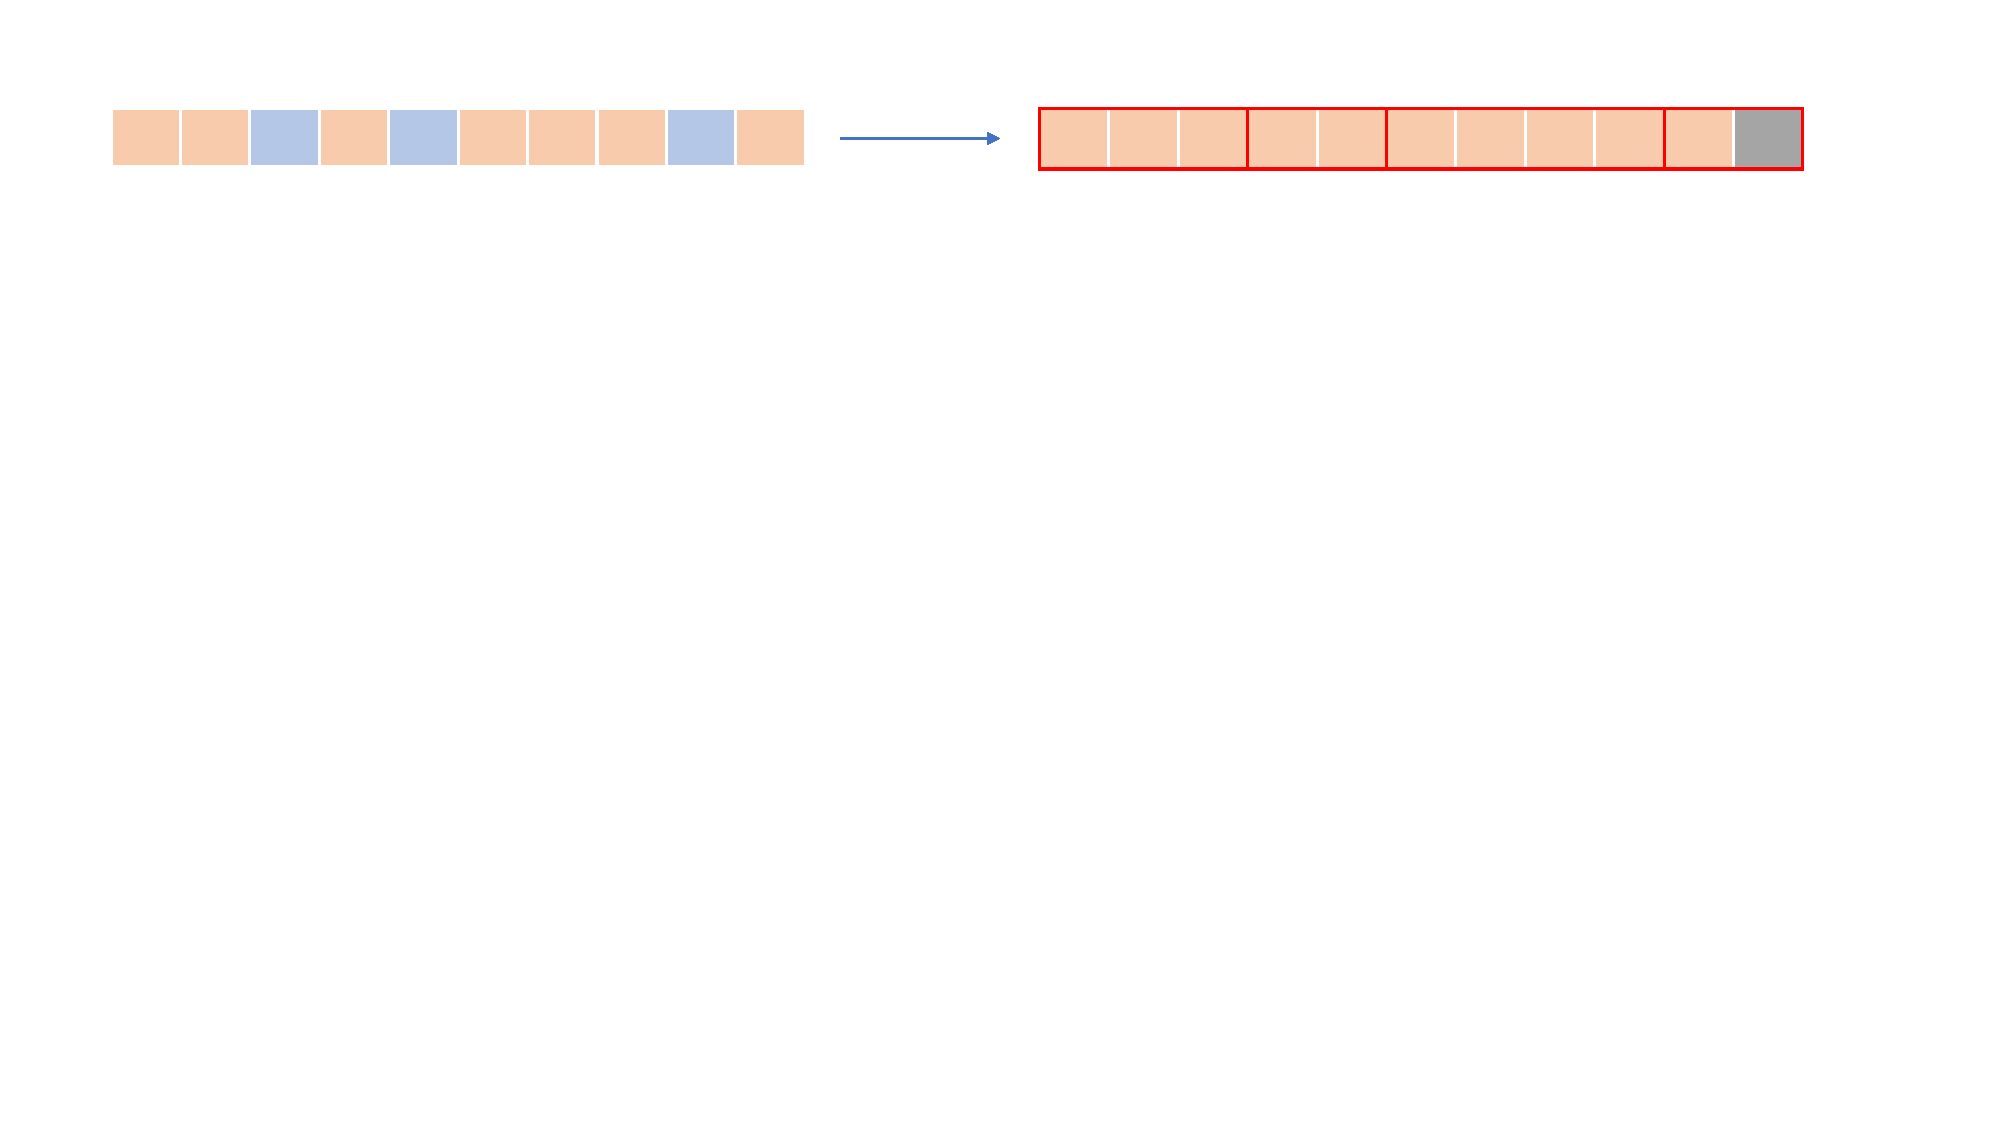
\includegraphics[width=0.8\textwidth]{./Figures/dummy_seat.pdf}
    \caption{Problem Conversion with One Seat as Social Distancing}
\end{figure}

After the conversion, $L = L^{0} + 1 =11$, $n_i = i + 1$ for $i = 1, 2, 3, 4$. For the first group, we use a group of three seats to indicate the original group of two and one seat used as the social distancing. We do the same procedure for the other groups. Then, the row can be represented by $\bm{h} = (2,1,1,0)$. The number of people that can be accommodated is $|\bm{h}| = 7$.

\end{example}

% We also introduce the concept of loss, which is the number of unoccupied seats. Mathematically, the loss is defined as $L- \delta - |\bm{h}|$, where $L$ denotes the length of the row.

\begin{definition}
Given the length of a row, denoted as $L$, and the maximum size of a group allowed, denoted as $M$, we can define certain characteristics of a pattern $\bm{h} = (h_1, \ldots, h_M)$.
We refer to a pattern $\bm{h}$ as a full pattern if it satisfies the condition $\sum_{i=1}^{M} n_i h_i = L$. Furthermore, we define a pattern $\bm{h}$ as a largest pattern if it has a size $|\bm{h}|$ that is greater than or equal to the size $|\bm{h}^{\prime}|$ of any other feasible pattern $\bm{h}^{\prime}$.
\end{definition}

In other words, a full pattern is one in which the sum of the product of the number of occurrences $h_i$ and the size $n_i$ of each group in the pattern is equal to the length of the row $L$. This ensures that the pattern fully occupies the available row seats. A largest pattern is one that either has the maximum size or is equal in size to other patterns, ensuring that it can accommodate the most number of people within the given row length.


\begin{prop}\label{lem_pattern}
Given the parameters of a row, including its length $L$, the social distancing requirement $\delta$, and the maximum size of a group allowed $M$, for one possible largest pattern $\bm{h}$, the maximum number of people that can be accommodated is given by $|\bm{h}| = qM + \max\{r-\delta, 0\}$, where $q = \lfloor \frac{L}{M + \delta} \rfloor$, $r \equiv L \bmod (M + \delta)$. 
\end{prop}

% The corresponding loss of the largest pattern equals $q \delta - \delta + \min\{r, \delta\}$, represents the amount of empty seats due to the social distancing requirement. 

The largest pattern $\bm{h}$ is unique and full when $r = 0$, indicating that only one pattern can accommodate the maximal number of people. On the other hand, if $r > \delta$, the largest pattern $\bm{h}$ is full, as it utilizes the available space up to the social distancing requirement.


\begin{example}
Consider the given values: $\delta = 1$, $L = 21$, and $M = 4$. In this case, we have $n_i = i + 1$ for $i = 1, 2, 3, 4$. The size of the largest pattern can be calculated as $qM + \max\{r-\delta, 0\} = 4 \times 4 + 0 = 16$. The largest patterns are the following: $(1, 0, 1, 3)$, $(0, 1, 2, 2)$, $(0, 0, 0, 4)$, $(0, 0, 4, 1)$, and $(0, 2, 0, 3)$.

The following figure shows that the largest pattern may not be full and the full pattern may not be largest.
\begin{figure}[ht]
    \centering
        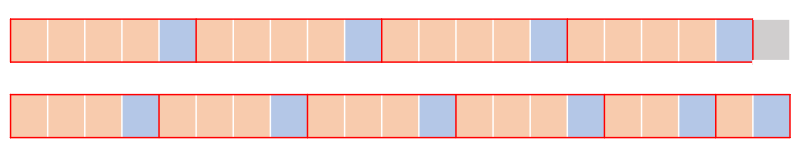
\includegraphics[width=0.8\textwidth]{./Figures/full_largest.png}
    \caption{Full and Largest Pattern}
\end{figure}

The first row can be represented by $(0, 0, 0, 4)$. It is a largest pattern as it can accommodate the maximum number of individuals. However, it does not satisfy the requirement of fully utilizing all available seats since $4 \times 5 \neq 21$.
The second row can be represented by $(1, 1, 4, 0)$, which is a full pattern as it utilizes all available seats. However, its size is 15, indicating that it is not the largest pattern.
\end{example}


Let $x_{ij}$ represent the number of group type $i$ planned in row $j$. The deterministic seat planning problem is formulated below, with the objective of maximizing the number of people accommodated.

\begin{equation}\label{deter_upper}
    \begin{aligned}
    \max \quad & \sum_{i=1}^{M}  \sum_{j= 1}^{N} (n_i- \delta) x_{ij} \\
    \text {s.t.} \quad & \sum_{j= 1}^{N} x_{ij} \leq d_{i}, \quad i \in \mathcal{M}, \\
    & \sum_{i=1}^{M} n_{i} x_{ij} \leq L_j, j \in \mathcal{N}, \\
    & x_{ij} \in \mathbb{Z}^{+}_{0}, \quad i \in \mathcal{M}, j \in \mathcal{N}.
    \end{aligned}
  \end{equation}
  
This seat planning problem can be regarded as a special case of the multiple knapsack problem. In this context, we define $\bm{X}$ as the aggregate solution, where $\bm{X} = (\sum_{j=1}^{N} x_{1j}, \ldots, \sum_{j=1}^{N} x_{Mj})^T$. Each element of $\bm{X}$, $\sum_{j=1}^{N} x_{ij}$, represents the available supply for group type $i$.
  
In other words, $\bm{X}$ captures the number each group type that can be allocated to the seat layout by summing up the supplies across all rows. By considering the monotone ratio between the original group sizes and the adjusted group sizes, we can determine the upper bound of supply corresponding to the optimal solution of the LP relaxation of Problem \eqref{deter_upper}, as demonstrated in Proposition \ref{sol_relax_deter}.

Although the problem size is small and the optimal solution can be easily obtained using a solver, it is still important to analyze the problem further to gain additional insights and understanding.

In many cases, the optimal solution for the seat planning problem tends to involve rows with either full patterns or the largest patterns. Distinguishing these patterns from other configurations can provide valuable insights into effective seat planning strategies that prioritize accommodating as many people as possible while adhering to social distancing guidelines.

When there is high demand for seats, it is advantageous to prioritize the largest patterns. These patterns allow for the accommodation of the largest number of individuals due to social distancing requirements. On the other hand, in scenarios with moderate demand, adopting the full pattern becomes more feasible. The full pattern maximizes seating capacity by utilizing all available seats, except those empty seats needed for social distancing measures. By considering both the largest and full patterns, we can optimize seat planning configurations to efficiently accommodate a significant number of individuals while maintaining adherence to social distancing guidelines. 
  

Although the optimal solution to the seat planning problem is complex, the LP relaxation of problem \eqref{deter_upper} has a nice property.

\begin{prop}\label{sol_relax_deter}
In the LP relaxation of problem \eqref{deter_upper}, there exists an index $\tilde{i}$ such that the optimal solutions satisfy the following conditions:

\begin{itemize}
\item For $i = 1,\ldots, \tilde{i}-1$, $x_{ij}^{*} = 0$ for all rows, indicating that no group type $i$ are assigned to any rows before index $v$.
\item For $i = \tilde{i}+1,\ldots, M$, the optimal solution assigns $\sum_{j} x_{ij}^{*} = d_{i}$ group type $i$ to meet the demand for group type $i$.
\item For $i = \tilde{i}$, the optimal solution assigns $\sum_{j} x_{ij}^{*} = \frac{L - \sum_{i = \tilde{i}+1}^{M} {d_i n_i}}{n_{\tilde{i}}}$ group type $\tilde{i}$ to the rows. This quantity is determined by the available supply, which is calculated as the remaining seats after accommodating the demands for group types $\tilde{i}+1$ to $M$, divided by the size of group type $\tilde{i}$, denoted as $n_{\tilde{i}}$.
\end{itemize}

Hence, the corresponding supply values can be summarized as follows: $X_{\tilde{i}} = \frac{L - \sum_{i = \tilde{i}+1}^{M} {d_i n_i}}{n_{\tilde{i}}}$, $X_{i} = d_{i}$ for $i = \tilde{i} +1,\ldots, M$, and $X_{i} = 0$ for $i = 1, \ldots, \tilde{i}-1$. These supply values represent the allocation of seats to each group type.
\end{prop}

\subsection{Generate The Seat Planning Composed of Full or Largest Patterns}
Given a specific pattern, we can convert it into a largest or full pattern while ensuring that the original group type requirements are met. When multiple full patterns are possible, our objective is to generate the pattern with minimal loss. Mathematically, for any pattern $\bm{h} = (h_1, \ldots, h_M)$, we seek to find a pattern $\bm{h}^{'} = (h_1^{'}, \ldots, h_M^{'})$ that maximizes $|\bm{h}^{'}|$ while satisfying the following constraints: $h_M{'} \geq h_M$, $h_{M-1}^{'} + h_{M}^{'} \geq h_{M-1} + h_{M}$, $\cdots$, $h_1^{'} + \ldots + h_M^{'} \geq h_1 + \ldots + h_M$. In other words, we want to find a pattern $\bm{h}^{'}$ where each element $h_i^{'}$ is greater than or equal to the corresponding element $h_i$ in $\bm{h}$, and the cumulative sums of the elements in $\bm{h}^{'}$ are greater than or equal to the cumulative sums of the elements in $\bm{h}$.
By finding such a pattern $\bm{h}^{'}$, we can ensure that the converted pattern meets or exceeds the requirements of the original group types. Among the possible full patterns that satisfy these constraints, we prioritize the one with the smallest loss.

Now, we demonstrate the specific allocation scheme.
Let $\beta_{j}= L_{j} - \sum_{i} n_{i} x_{ij}$. If row $j$ is not the largest or full, then $\beta_{j} > 0$. 
We aim to allocate the remaining unoccupied seats in row $j$ in a way that maximizes the number of planned groups that become the largest in size. Find the smallest group type in the pattern denoted as $k$. If $k = M$, it means that this row corresponds to a largest pattern. If $k \neq M$, we reduce the number of group type $k$ by one and increase the number of group type $\min \{(k+\beta_{j}), M\}$ by one, the number of unoccupied seats will be reduced correspondingly.

We continue this procedure until either all the planned groups become the largest or $\beta_{j} = 0$. If $\beta_{j} = 0$, it indicates that the pattern is full. In this case, we have assigned all the unoccupied seats to the existing groups without incurring any additional loss. Therefore, this full pattern has the minimal loss while satisfying the groups requirement. However, if all the planned groups become the largest and $\beta_{j} \neq 0$, we can repeatly follow the steps outlined below to obtain the largest pattern:

\begin{itemize}
  \item If $\beta_{j} \geq n_{M}$, we can assign $n_M$ seats to a new group type $M$.

  \item If $n_{1} \leq \beta_{j} < n_{M}$, we can assign $\beta_{j}$ seats to a new group type $\beta_{j}-n_{1}+1$.
  \item If $0 < \beta_{j} < n_{1}$, it means that the current pattern is already the largest possible pattern because all the planned groups in the pattern are the largest.
\end{itemize}

By following these steps and always prioritizing the largest group type for seat planning, we can achieve either the largest pattern or a full pattern with minimal loss. This approach guarantees efficient seat allocation, maximizing the utilization of available seats while still accommodating the original groups' requirements.

To construct the largest or full pattern for each row, we can employ the following algorithm. Since patterns are independent of each other, we can process them row by row within a given seat planning. This enables us to optimize the seat planning by maximizing the utilization of available seats and effectively accommodating the arriving groups.

\begin{algorithm}
  \caption{Construct The Largest or Full Pattern}\label{construction}
  % \KwIn{Pattern $\bm{h}$}
  % \KwOut{Pattern}
  \While{$\beta > 0$}
    {$k \gets \min_{i}\{h_{i} \neq 0\}$\Comment*[r]{Find the smallest group type in the pattern}
    \eIf{$k \neq M$}
    {$h_{k} \gets h_{k} - 1$\; $h_{\min\{k+\beta, M\}} \gets h_{\min\{k+\beta, M\}} + 1$\;
    $\beta \gets \beta - \max\{1, M - k\}$\Comment*[r]{Change the current group type to a group type as large as possible}}
    {\eIf{$\beta \geq n_{M}$}
    {$q \gets \lfloor\frac{\beta}{n_M}\rfloor$\;
     $\beta \gets \beta - q n_M$\; $h_{M} \gets h_{M} + q$\Comment*[r]{Assign seats to as many the largest group type as possible}}
    {\eIf{$n_{1} \leq \beta < n_{M}$}
    {$h_{\beta-n_1+1} \gets h_{\beta-n_1+1} + 1$\; $\beta \gets 0$\;}
    {$\bm{h}$ is the largest\; $\beta \gets 0$\;}}
    }}
\end{algorithm}


% \subsection{Dynamic Seat Assignment with Social Distancing}\label{sec_dynamic_seat}
% In a more realistic scenario, groups arrive sequentially over time, and the seller must promptly make group assignments upon each arrival while maintaining the required spacing between groups. When a group is accepted, the seller must also determine which seats should be assigned to that group. It is essential to note that each group must be either accepted in its entirety or rejected entirely; partial acceptance is not permitted. Once the seats are confirmed and assigned to a group, they cannot be changed or reassigned to other groups.

% To model this problem, we adopt a discrete-time framework. Time is divided into $T$ periods, indexed forward from $1$ to $T$. We assume that in each period, at most one group arrives and the probability of an arrival for a group of size $i$ is denoted as $p_i$, where $i$ belongs to the set $\mathcal{M}$. The probabilities satisfy the constraint $\sum_{i=1}^M p_i \leq 1$, indicating that the total probability of any group arriving in a single period does not exceed one. We introduce the probability $p_0 = 1 - \sum_{i=1}^{M} p_i$ to represent the probability of no arrival in a given period $t$. To simplify the analysis, we assume that the arrivals of different group types are independent and the arrival probabilities remain constant over time. This assumption can be extended to consider dependent arrival probabilities over time if necessary.

% The state of remaining capacity in each row is represented by a vector $\mathbf{L} = (l_1, l_2, \ldots, l_N)$, where $l_j$ denotes the number of remaining seats in row $j$. Upon the arrival of a group type $i$ in period $t$, the seller needs to make a decision denoted by $u_{i,j}^{t}$, where $u_{i,j}^{t} = 1$ indicates acceptance of group type $i$ in row $j$ during period $t$, while $u_{i,j}^{t} = 0$ signifies rejection of that group type in row $j$ at that period. The feasible decision set is defined as $$U^{t}(\mathbf{L}) = \{u_{i,j}^{t} \in \{0,1\}, \forall i \in \mathcal{M}, \forall j \in \mathcal{N} | \sum_{j=1}^{N} u_{i,j}^{t} \leq 1, \forall i \in \mathcal{M}; n_{i}u_{i,j}^{t}\mathbf{e}_j \leq \mathbf{L}, \forall i \in \mathcal{M}, \forall j \in \mathcal{N}\}.$$ Here, $\mathbf{e}_j$ represents an N-dimensional unit column vector with the $j$-th element being 1, i.e., $\mathbf{e}_j = (\underbrace{0, \cdots, 0}_{j-1}, 1, \underbrace{0, \cdots, 0}_{n-j})$. In other words, the decision set $U(\mathbf{L})$ consists of all possible combinations of acceptance and rejection decisions for each group type in each row, subject to the constraints that at most one group of each type can be accepted in any row, and the number of seats occupied by each accepted group must not exceed the remaining capacity of the row.

% Let $V^{t}(\mathbf{L})$ denote the maximum expected revenue earned by the best decisions regarding group seat assignments in period $t$, given remaining capacity $\mathbf{L}$. Then, the dynamic programming formula for this problem can be expressed as:

% \begin{equation}\label{DP}
% V^{t}(\mathbf{L}) = \max_{u_{i,j}^{t} \in U^{t}(\mathbf{L})}\left\{ \sum_{i=1}^{M} p_i ( \sum_{j=1}^{N} i u_{i,j}^{t} + V^{t+1}(\mathbf{L}- \sum_{j=1}^{N} n_i u_{i,j}^{t}\mathbf{e}_j)) + p_0 V^{t+1}(\mathbf{L})\right\}
% \end{equation}
% with the boundary conditions $V^{T+1}(\mathbf{L}) = 0, \forall \mathbf{L}$ which implies that the revenue at the last period is 0 under any capacity.

% At the beginning of period $t$, we have the current remaining capacity vector denoted as $\mathbf{L} = (L_1, L_2, \ldots, L_N)$. Our objective is to make group assignments that maximize the total expected revenue during the horizon from period 1 to $T$ which is represented by $V^{1}(\mathbf{L})$.

% Solving the dynamic programming problem described in equation \eqref{DP} can be challenging due to the curse of dimensionality, which arises when the problem involves a large number of variables or states. To mitigate this complexity, we aim to develop a heuristic method for assigning arriving groups. In our approach, we begin by generating a seat planning that consists of the largest or full patterns, as outlined in section \ref{sec_seat_planning}. This initial seat planning acts as a foundation for our heuristic method. In section \ref{sec_dynamic_seat}, building upon the generated seat planning, we further develop a dynamic seat assignment policy which guides the allocation of seats to the incoming groups sequentially. 










